%!TEX root = *.tex
%%%%%%%%%%%%%%%%%%
% メモ
\begin{comment}

\end{comment}
% カウンタのリセット
\setcounter{eqNo}{0}
\setcounter{figure}{0}
% 解答
\noindent {\large【解答】\par}
\noindent (1)\,
電気容量$C\unit{F}$のコンデンサーの極板間電圧が$V\unit{V}$となるので,蓄えられているエネルギーは$\dfrac{1}{2}CV^2\unit{J}$.

\noindent (2)\,
Aの電位が$0\,\textup{V}$,Bの電位が$V\unit{V}$で,
AB間は一様な電場であるから,電位と位置のグラフは直線となる
(図1).

\noindent (3)\,
AB間の電場は一様であり,$V=Ed$より$E=\dfrac{V}{d}\unit{V/m}$で一定である(図2).

\noindent (4)\,
コンデンサー間に金属板を挿入すると,コンデンサーの極板間隔が小さくなると見なすことができる.
また,極板間隔$d$が半分になると,コンデンサーの容量$C=\epsilon_0 \dfrac{S}{d}$は2倍になるので,$2C\unit{F}$となる.
AB間の電位差はVなので,蓄えられている電気量$Q_2$は,
\begin{align*}
  Q_2 = 2C\cdot V = 2CV
\end{align*}

\noindent (5)\, 
挿入した金属板の内部は等電位で,電場の強さは0である.
Aの電位が$0\textup{V}$,Bの電位が$V\unit{V}$であるので,中央の金属板の電位は$\dfrac{1}{2}\unit{V}$.図示したものは図1.

\noindent (6)\,
極板と金属板の間の電場の強さ$E$は,
\begin{align*}
  E = \dfrac{V/2}{d/4} = \dfrac{2V}{d} \unit{V/m}
\end{align*}
である.金属板内の電場は0であることと合わせて図示して図2.

\noindent (7)\, 
AB間の電位差は$V$である.
誘電体は容量が$\epsilon_r\epsilon_0\dfrac{S}{d/2}=4C$であるコンデンサーとみなせる.極板と誘電体の間も容量$4C$のコンデンサーである.
よって,電気容量$4C$のコンデンサーが3つ直列接続されている合成容量$C_3$は
\begin{align*}
  \dfrac{1}{C_3} = \dfrac{1}{4C} + \dfrac{1}{4C} + \dfrac{1}{4C} = \dfrac{3}{4C}\\
  \therefore C_3 = \dfrac{4}{3}C
\end{align*}
よって,蓄えられている電気量$Q_3$は
\begin{align*}
  Q_3 = \dfrac{4}{3}C\cdot V = \dfrac{4}{3}CV\unit{C}
\end{align*}

\noindent (8)\, 
極板Aと誘電体の左端の電位差を$V_l\unit{V}$とすると,
\begin{align*}
  V_l = \dfrac{Q_3}{4C} = \dfrac{1}{3}V\unit{V}
\end{align*}
同様に,極板Bと誘電体の右端の電位差を$V_r=\dfrac{1}{3}\unit{V}$.
また,誘電体の両端間の電位差$V_c$は,
\begin{align*}
  V_c = \dfrac{Q_3}{4C} = \dfrac{1}{3}V\unit{V}
\end{align*}

\noindent (9)\,
それぞれの電位の強さ$E_l,\,E_c,\,E_r$は,
\begin{align*}
  E_l &= E_r = \dfrac{V/3}{d/4} = \dfrac{4V}{3d} \\
  E_c &= \dfrac{2V}{3d}
\end{align*}

\noindent (10)\, 
スイッチを開いても電荷は保存される.
誘電体が挿入されていたとき,蓄えられていた
電気量$Q_3=\dfrac{4}{3}CV\unit{C}$であり,容量は$C_3=\dfrac{4}{3}C\unit{F}$であったので,
蓄えられていた静電エネルギー$U$は
\begin{align*}
  U = \dfrac{{Q_3}^2}{2{C_3}} = \dfrac{2}{3}CV^2\unit{J}
\end{align*}
ここで,誘電体を取り除いた後の電気容量は$C\unit{F}$なので
静電エネルギー$U^\prime$は
\begin{align*}
  U^\prime = \dfrac{{Q_3}^2}{2C} = \dfrac{8}{9}CV^2\unit{J}
\end{align*}
となる.
よって,誘電体を取り除くのに要した仕事$W$は静電エネルギーの増加分にあたり,
\begin{align*}
  W = U^\prime-U = \dfrac{2}{9}CV^2\unit{J}
\end{align*}

\noindent (11)\, 
極板間隔を$\dfrac{3}{2}$倍に広げると電気容量は$\dfrac{2}{3}$倍になる.
電荷が保存されるので,AB間の電位差$V_4$は
\begin{align*}
  V_4 = \dfrac{Q_3}{(2/3)C} = 2V\unit{V}
\end{align*}

\begin{figure}[htbp]
  \centering
  \begin{minipage}{0.4\columnwidth}
    \centering
    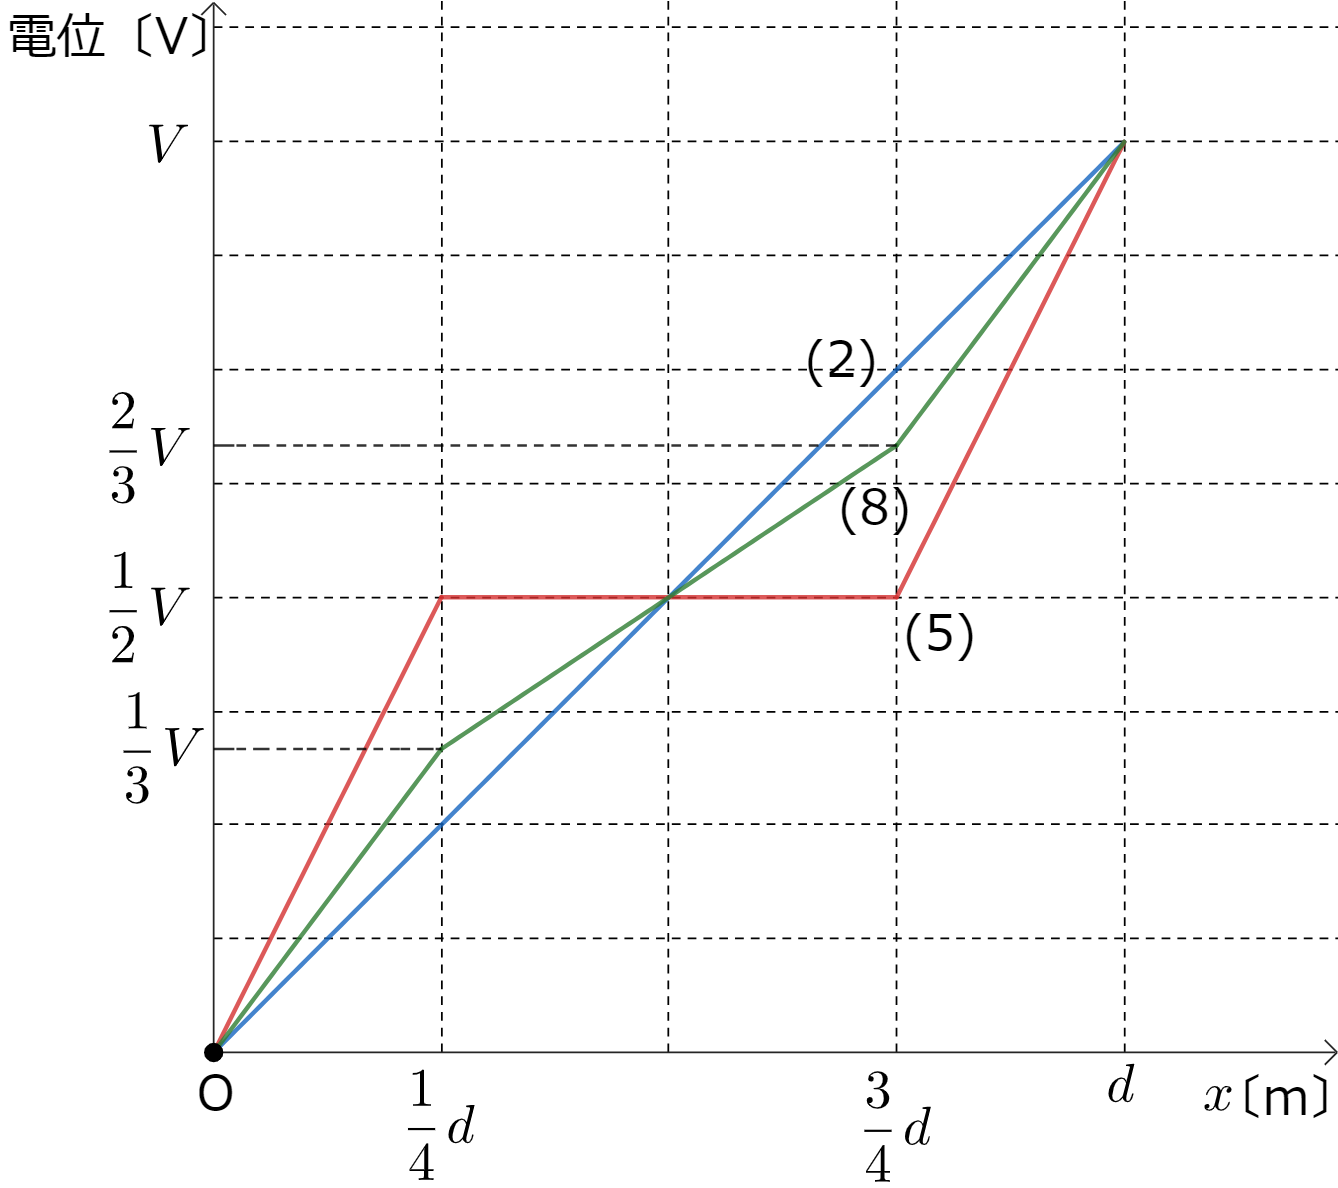
\includegraphics[width=\columnwidth]{../graphs/jumon_108_sol_2.png}
    \caption{}
  \end{minipage} 
  \begin{minipage}{0.4\columnwidth}
    \centering
    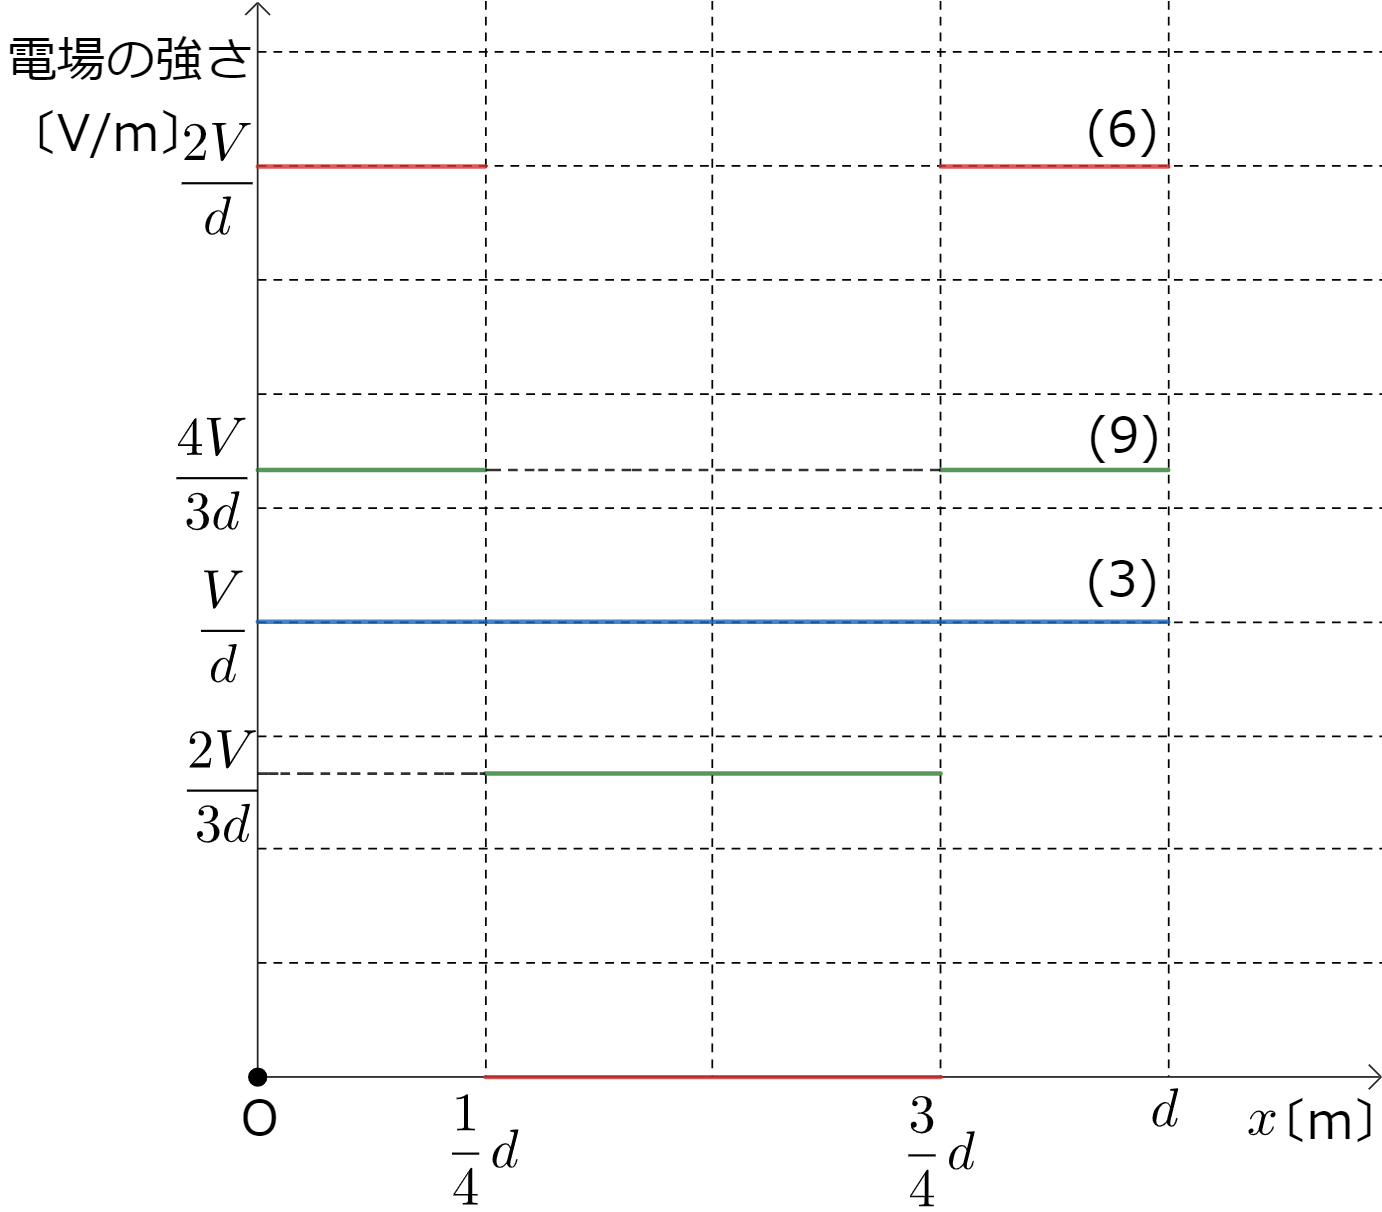
\includegraphics[width=\columnwidth]{../graphs/jumon_108_sol_3.png}
    \caption{}
  \end{minipage}
\end{figure}


%%%%%%%%%%%%%%%%%%
